\documentclass[letterpaper]{article}
\usepackage{natbib,alifexi}
\usepackage[bordercolor=gray!20,backgroundcolor=blue!10,linecolor=blue,textsize=footnotesize,textwidth=0.8in]{todonotes}
\usepackage{hyperref}
\usepackage{algpseudocode}
\usepackage{algorithm}
\usepackage{subfig}

\title{Meta Reinforcement Learning for Constant Continuous Reward Tasks}
\author{Florentin Hennecker \\
\mbox{}\\
Universit\'e Libre de Bruxelles, Boulevard du Triomphe - CP 212, 1050
Brussels, Belgium \\
fhenneck@ulb.ac.be}

\marginparwidth=0.5in
\newcommand\Tstrut{\rule{0pt}{2.6ex}}
\newcommand\Bstrut{\rule[-0.9ex]{0pt}{0pt}}


\begin{document}
\maketitle

\begin{abstract}
	Meta reinforcement learning recently emerged as the art of teaching
	an agent to learn to solve a task as opposed to teaching an agent
	to solve a task. The generalisation capabilities of meta-learning
	agents and their very fast learning feats have been tested on 
	multi-armed bandit problems as well as visual navigation tasks. This
	paper enables the use of a meta-learning setup on continuous state-space
	problems such as Acrobot and CartPole with a constant timestep-based 
	reward using simple reward shaping. The performance of this setup
	is tested on a distribution of parametrised Acrobot environments and
	tampered state observation vectors.
\end{abstract}

\section{Introduction}
There have been incredible advances in the field of reinforcement learning
in the past few years. Deep Q-learning \citep{dqn, dqn_nature} made learning Atari
games from visual inputs possible, even beating the human level benchmark
for some games; less than two years later, a similar milestone has been reached
for playing Doom, a complex 3D game \citep{doom} using the VizDoom environment
\citep{vizdoom}. Most of these achievements share one issue: once the agents
described in these papers have learned to solve the task they were handed,
they are likely to fail on slightly different versions of the task and will
have to be completely retrained for new tasks, however similar they are from
the task the agent was trained on.

Just like humans use prior knowledge to quickly learn new tasks that are
presented to them, training an agent to learn to solve variations of a problem
is unlikely to be possible without giving it some sort of prior knowledge.
A second key component needed for a fast-learning agent would be a good
learning strategy (\textit{in the sense where $\epsilon$-greedy or softmax selection
\citep{suttonbarto}, Q-learning \citep{qlearning} and SARSA \citep{sarsa} 
are learning strategies})
that takes into account prior knowledge and takes action
to learn about the problem as fast as it can to perform optimally as
soon as possible.

\begin{figure}[H]
	\centering
	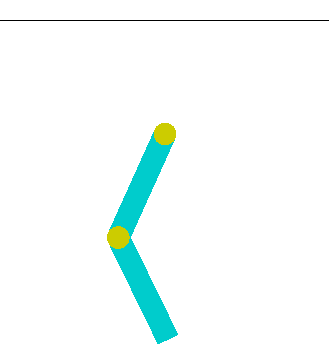
\includegraphics[width=.4\linewidth]{fig/acrobot.png}
	\caption{The Acrobot environment}
	\label{fig:acrobot}
\end{figure}


Finding such a strategy is hard, but it can be cast as a reinforcement
learning problem: instead of designing a learning strategy by hand and
teaching the agent to solve a task, \cite{learningtorl}
and \cite{fastrlviaslowrl} propose to
teach an agent to learn to solve a task. The agent presented by Wang et al. is 
an A2C (a single-threaded version of A3C \citep{a3c})
agent with a recurrent connection and presents
two major differences compared to a standard reinforcement learning agent: 
\begin{enumerate}
	\item the agent is trained on trials of episodes rather than on single
		episodes, replicating the training process in standard 
		reinforcement learning
	\item the agent receives process-level information as well as
		an observation of the enviromnent: the reward at the previous
		timestep, the action that led to that reward and an 
		episode termination flag.
\end{enumerate}

Conceptually, in standard reinforcement learning, the network represents 
a policy and its goal is to collect an optimal reward for one episode. In
meta reinforcement learning, the network represents an algorithm which
learns a policy. Its weights, once trained, encode a learning strategy which
decides how to play episodes to maximise reward across multiple episodes.


\begin{figure*}[h]
	\centering
	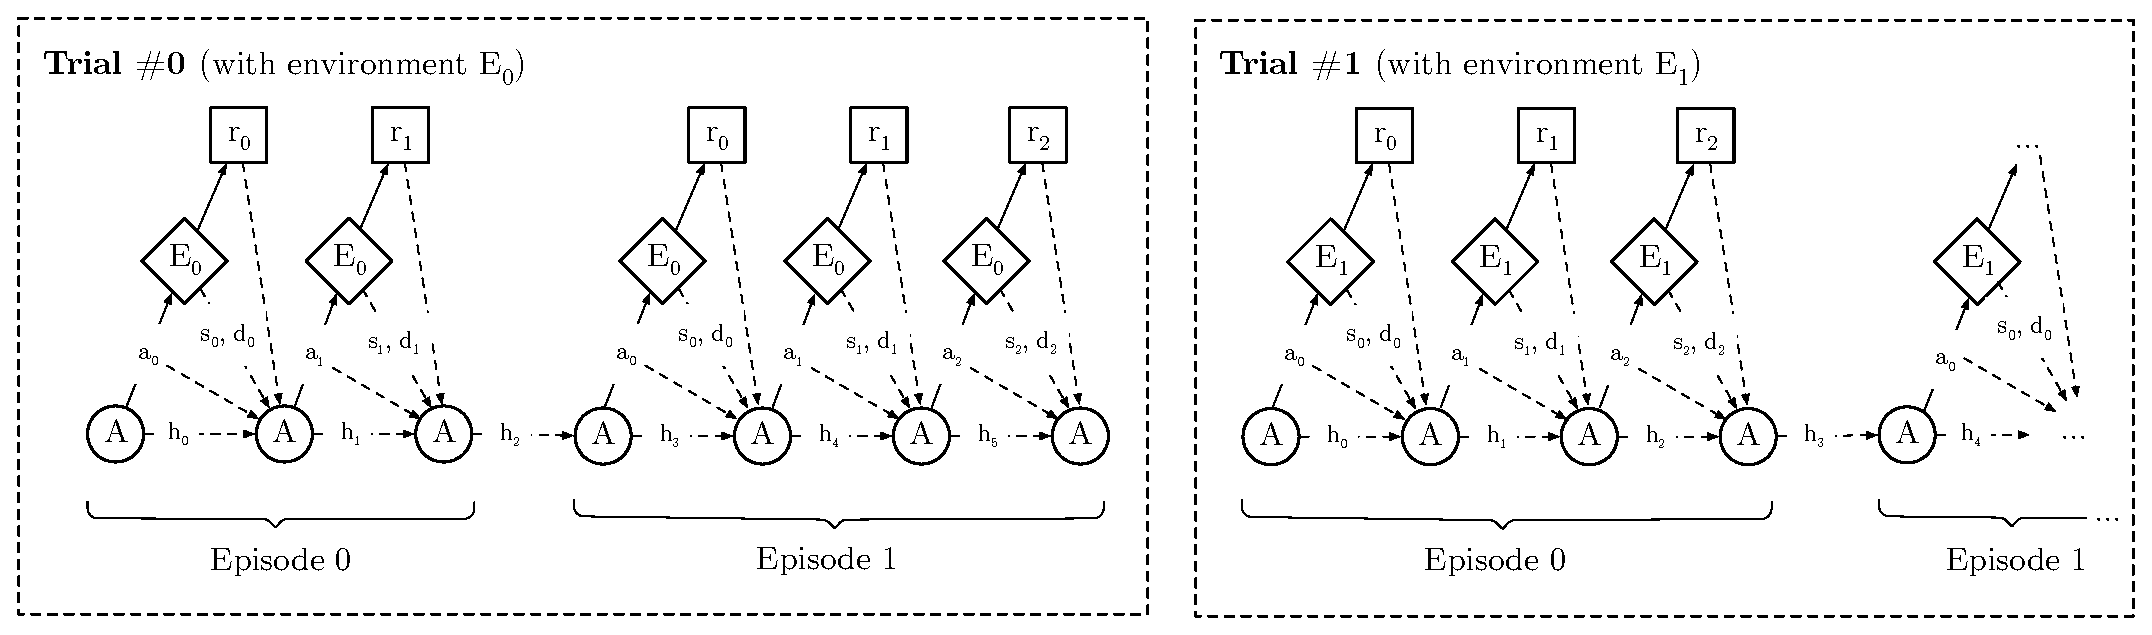
\includegraphics[width=\textwidth]{fig/meta_learning_process.eps}
	\caption{The process of training a meta-learning agent. 
	A is the agent, E is the environment. At each
	timestep, it receives the state of the environment $s_t$, 
	the previous action taken $a_{t-1}$, the reward of the previous
	transition $r_{t-1}$ and an episode termination flag $d_{t-1}$ set to 1 is the
	state is terminal, 0 otherwise.}
	\label{fig:meta_learning_process}
\end{figure*}


\begin{figure}[h]
	\centering
	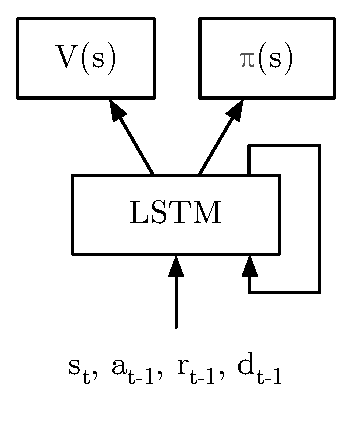
\includegraphics[width=.4\linewidth]{fig/a2c_meta.eps}
	\caption{The architecture of the meta-learning agent as presented in
	\cite{learningtorl} with a LSTM instead of a GRU cell.}
	\label{fig:a2c}
\end{figure}

Both Wang et al. and Duan et al. show convincing learning behaviour from
the meta-learning agent in various types of bandit problems but also
a complex visual navigation task \citep{learningtonavigate}. In both situations, 
the agent deploys a strategy that performs excellent exploration based on its 
prior knowledge of the structure of the task 
and then exploits the knowledge gained during exploration to perform 
optimally for the following episodes. In situations where it is possible, the
agent is able to perform one-shot learning.

We will apply meta reinforcement learning to a new class of problems with
continuous state spaces and a timestep-based-only reward, generating 
a distribution of similar tasks by modifying some intrinsic parameters
of the Acrobot environment such as the length and mass of the links, but also
by tampering with the observation vector obtained by the agent.

\subsection{Background} 
The meta-learning A2C agent presented in \cite{learningtorl} is a recurrent
neural network with two outputs; a policy output (the actor) and a value
output (the critic). Its input is not only the state of the environment $s_t$,
but also the previous action taken $a_{t-1}$, the reward of the previous
transition $r_{t-1}$ and an episode termination flag $d_{t-1}$ set to 1 is the
state is terminal, 0 otherwise. \cite{learningtorl} use a GRU \citep{grus} cell
for the recurrent part of the architecture; we use a 48 unit LSTM cell 
\citep{lstm}. Figure~\ref{fig:a2c} shows the architecture of our agent.

The agent is trained to play \textbf{trials} of several episodes, and its
hidden state is passed along even inbetween different episodes, but not
between trials (see Figure~\ref{fig:meta_learning_process}). Its goal is to 
maximise its reward across all episodes of a trial.

The loss of the A2C agent is the following : 
$$ \mathcal{L} = \beta_v \mathcal{L}_v + \beta_p \mathcal{L}_p - \beta_e 
 \mathcal{L}_e $$
where $\mathcal{L}_v$ is the value loss : 
$$ \mathcal{L}_v = (R_{t-1} - V(s_t))^2$$
$\mathcal{L}_p$ is the policy loss : 
$$ \mathcal{L}_p = \pi(a_t \mid s_t) (R_t - V(s_t))$$
$\mathcal{L}_e$ is the entropy regularisation : 
$$ \mathcal{L}_e = \sum\limits_{a \in A}\pi(a \mid s_t)\log(\pi(a \mid s_t))$$
where 
$$R_t = \sum\limits_{k=0}^{\infty} \gamma^k r_{t+k}$$

In our experiments, we use $\gamma = 0.97$, $\beta_v = 0.5$, $\beta_p = 1$, 
$\beta_e = 0.05$. An update is performed
once after every trial using Adam \citep{adam} with a learning rate of 0.001.\\



\section{Methods}
We will apply the meta-learning setup presented in \cite{learningtorl} and
\cite{fastrlviaslowrl} to a distribution of continuous state problems with a 
constant reward at each timestep. This distribution will be derived from
the original Acrobot problem \citep{acrobot1996, acrobot2015}. The Acrobot
environment (illustrated in Figure~\ref{fig:acrobot}) consists of two links 
that are connected with an actuated joint. The upper link is fixed with an 
unactuated joint. The goal of the agent is to swing the lower link above a 
given height.

We generate a distribution of similar problems by modifying
two of the Acrobot parameters: the link lengths and their masses. The default
values for each of these is 1, but for each trial, we will sample uniformly:
\begin{itemize}
	\item a length $l \in \{0.5, 1, 2\}$ for each link;
	\item a mass $m \in \{0.1, 1\}$ for each link.
\end{itemize}

\subsubsection{Reward shaping}
Applying the setup presented by \cite{learningtorl} as is on the Acrobot
problem (and other problems with similar reward structures, e.g. the
CartPole problem \citep{barto-cartpole}) will generate unwanted episode-wise
reward dynamics. The reward structure of such problems is simple:
either +1 or -1 at every timestep. In human-designed learning strategies, the
designer knows that for a problem like Acrobot, a short episode is a good thing,
and this knowledge will be implicitly distilled in the learning strategy. 



This knowledge is not available to the meta-learning agent. In fact, it does
not have any incentive to finish episodes that are far from the trial horizon
as quickly as possible. This is due to the fact that the discount factor makes
the agent only take into account a limited number of timesteps away from a time
$t$. If the agent is playing the last episode, it can potentially see the
end of the constant -1 reward stream and take action to reach it; in the first
episodes, whatever the agent does, the negative reward stream will continue no 
matter how quickly it solved the problem. 


This is why we need to introduce a process-level reward, just like we feed
process-level information such as the episode termination flag, the reward
and previous action taken to the agent. For the Acrobot problem, we can
give the agent a small positive reward at the end of an episode to encourage
the agent to reach it as quickly as possible. All our experiments feed a
reward of +10 at the last timestep of each episode in a trial.\\

We will compare the performance of an agent trained on trials of 1 episode
and on 2 episodes to estimate the impact of letting the agent play one episode
after it has interacted with the environment and hopefully estimated
its parameters. This comparison will be conducted on different settings,
modifying the parameters of the game and introducing unseen behaviours of
the environment to evaluate the generalisation performance of both agents.

\begin{figure}[h!]
	\centering
	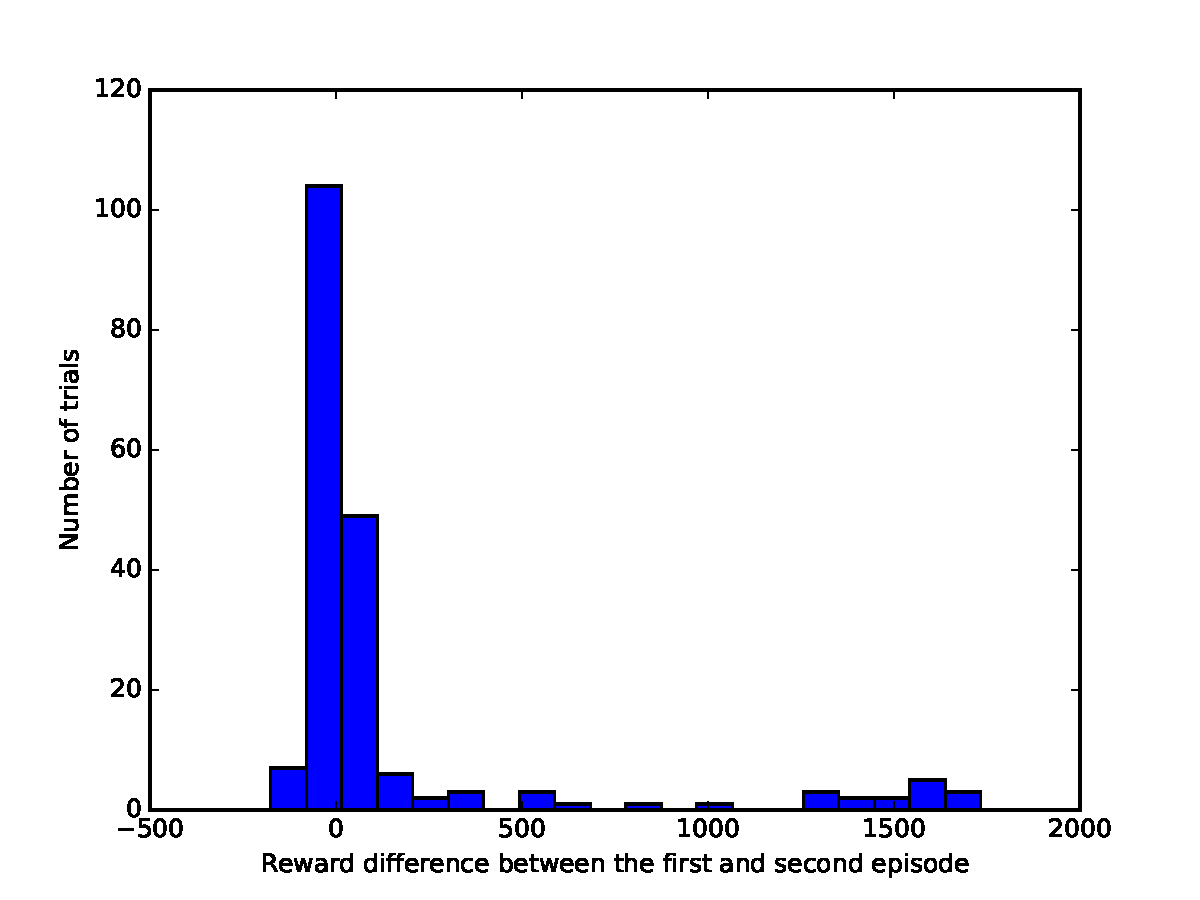
\includegraphics[width=\linewidth]{fig/reward_diff.pdf}
	\caption{Distribution of the reward difference between the first
	and the second episode of a dual-episode trial for experiment 1}
	\label{fig:reward_diff}
\end{figure}
\begin{figure}[h!]
	\centering
	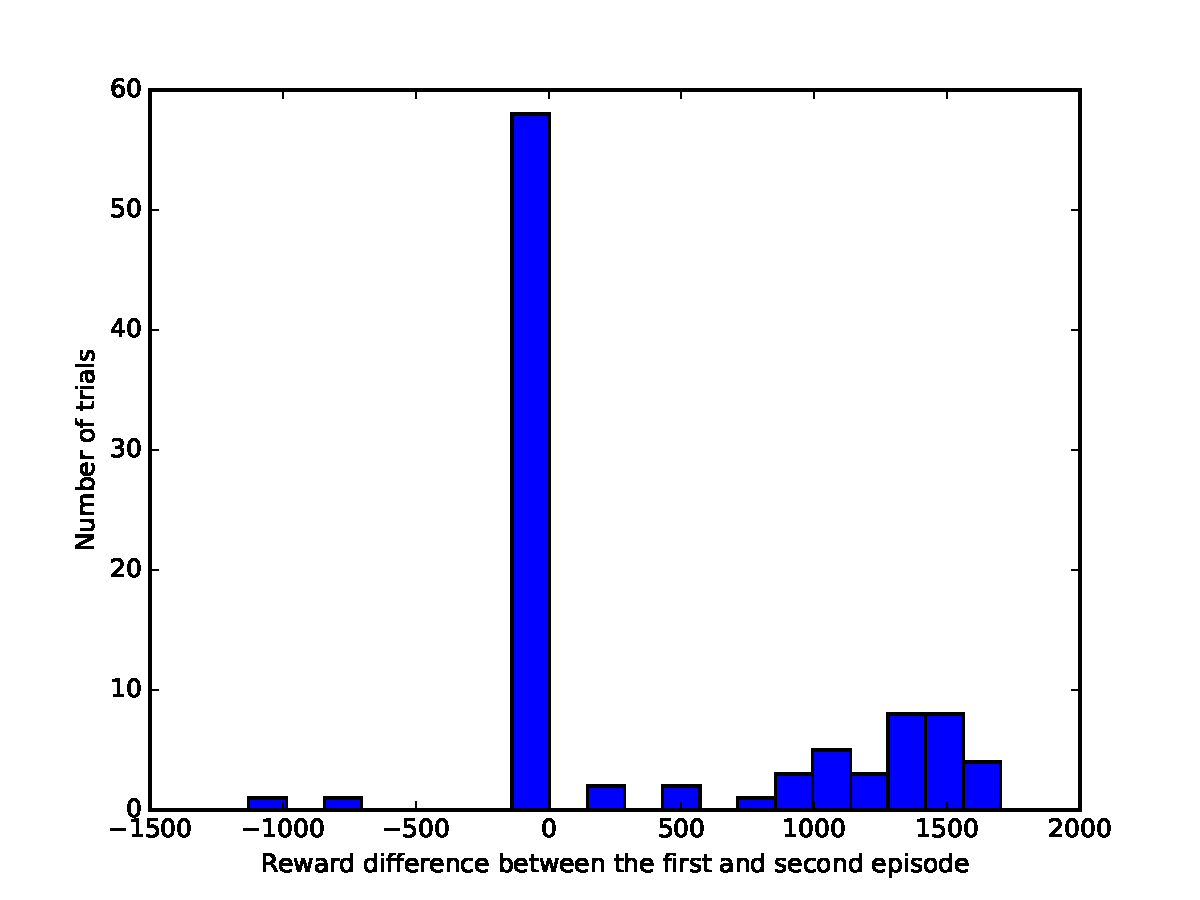
\includegraphics[width=\linewidth]{fig/reward_diff_cunseen.pdf}
	\caption{Distribution of the reward difference between the first
	and the second episode of a dual-episode trial for experiment 2}
	\label{fig:reward_diff_cunseen}
\end{figure}



\begin{figure*}[h!]
	\centering
	\subfloat[][Trials of 1 episode]{
		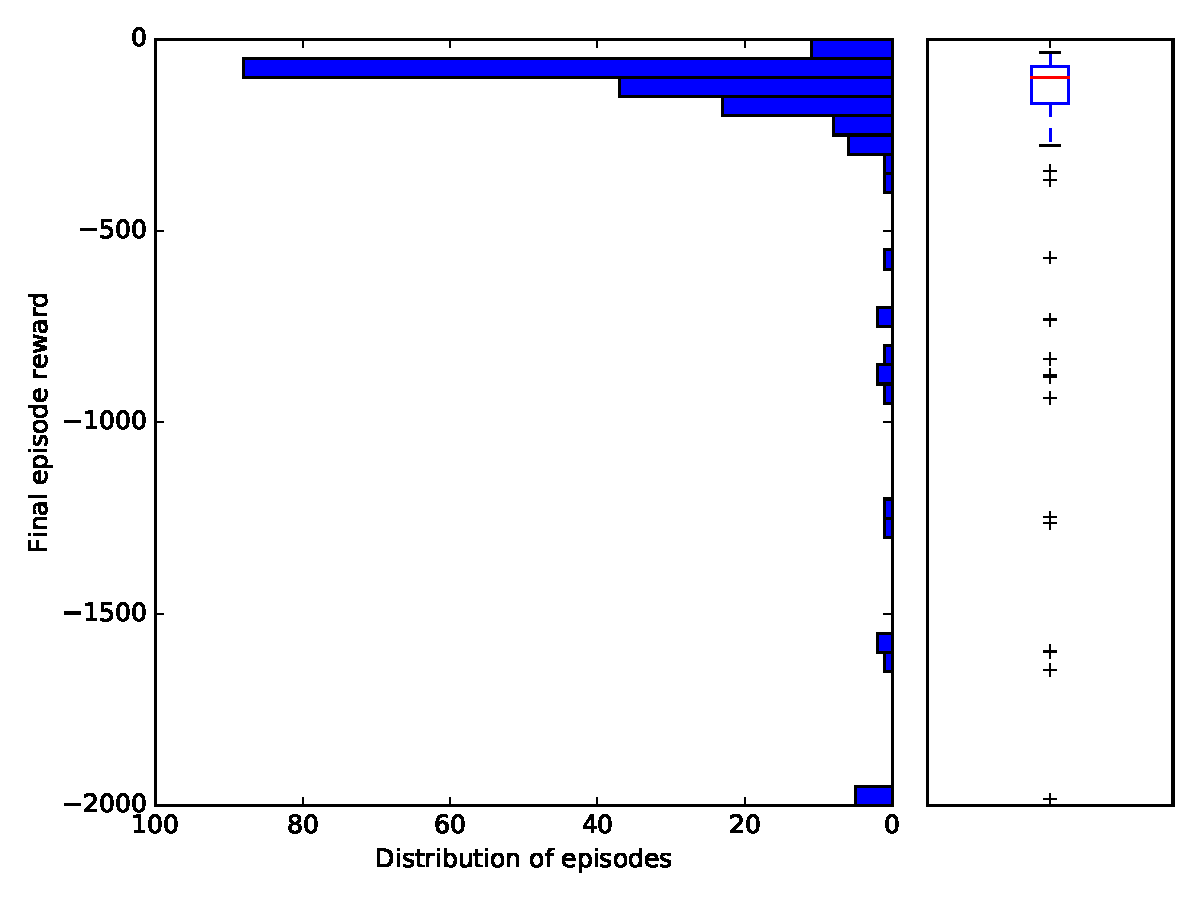
\includegraphics[width=0.49\linewidth]{fig/distrib1.pdf}}
	\subfloat[][Trials of 2 episode]{
		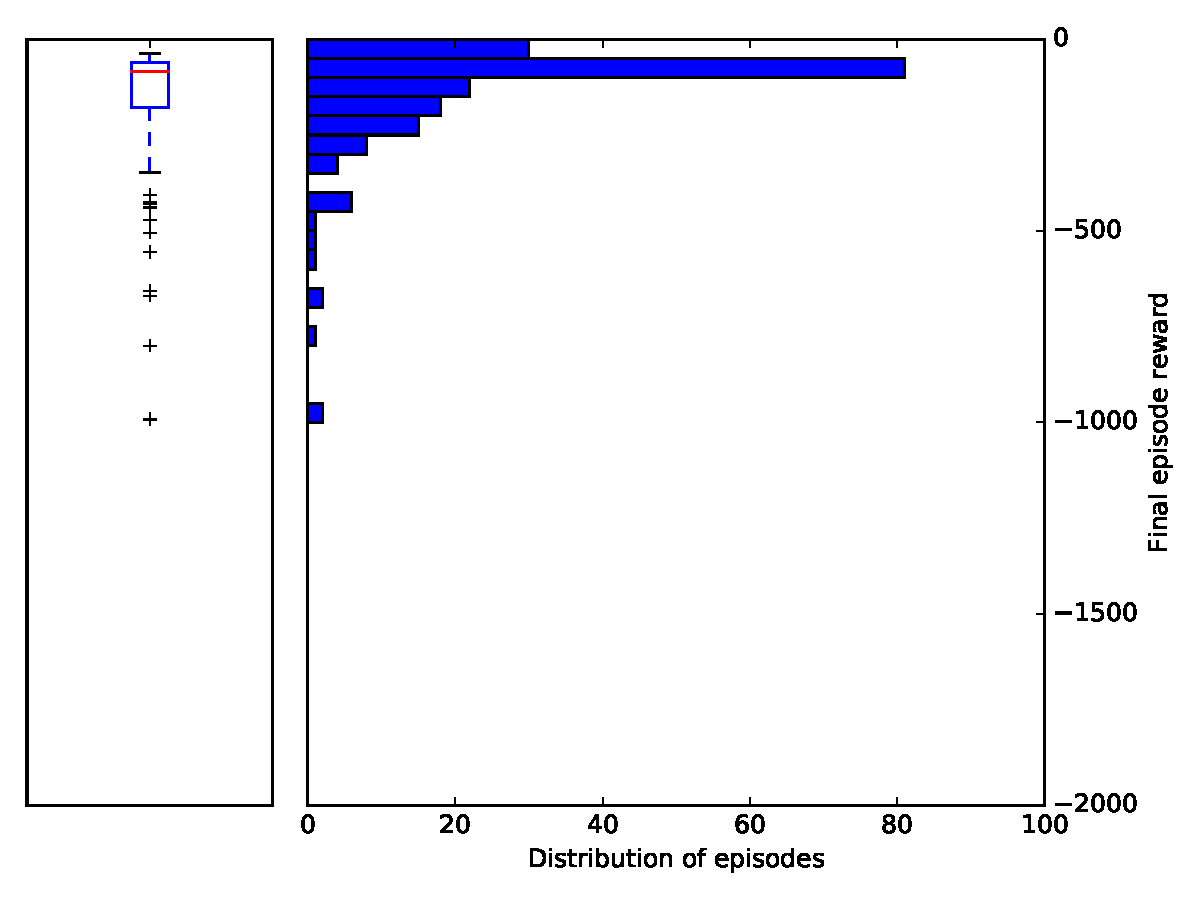
\includegraphics[width=0.49\linewidth]{fig/distrib2.pdf}}
	\caption{Distribution of the total reward obtained during final episodes
	for trials of different lengths for experiment 1}
	\label{fig:distrib}
\end{figure*}

\begin{figure*}[h!]
	\centering
	\subfloat[][Trials of 1 episode]{
		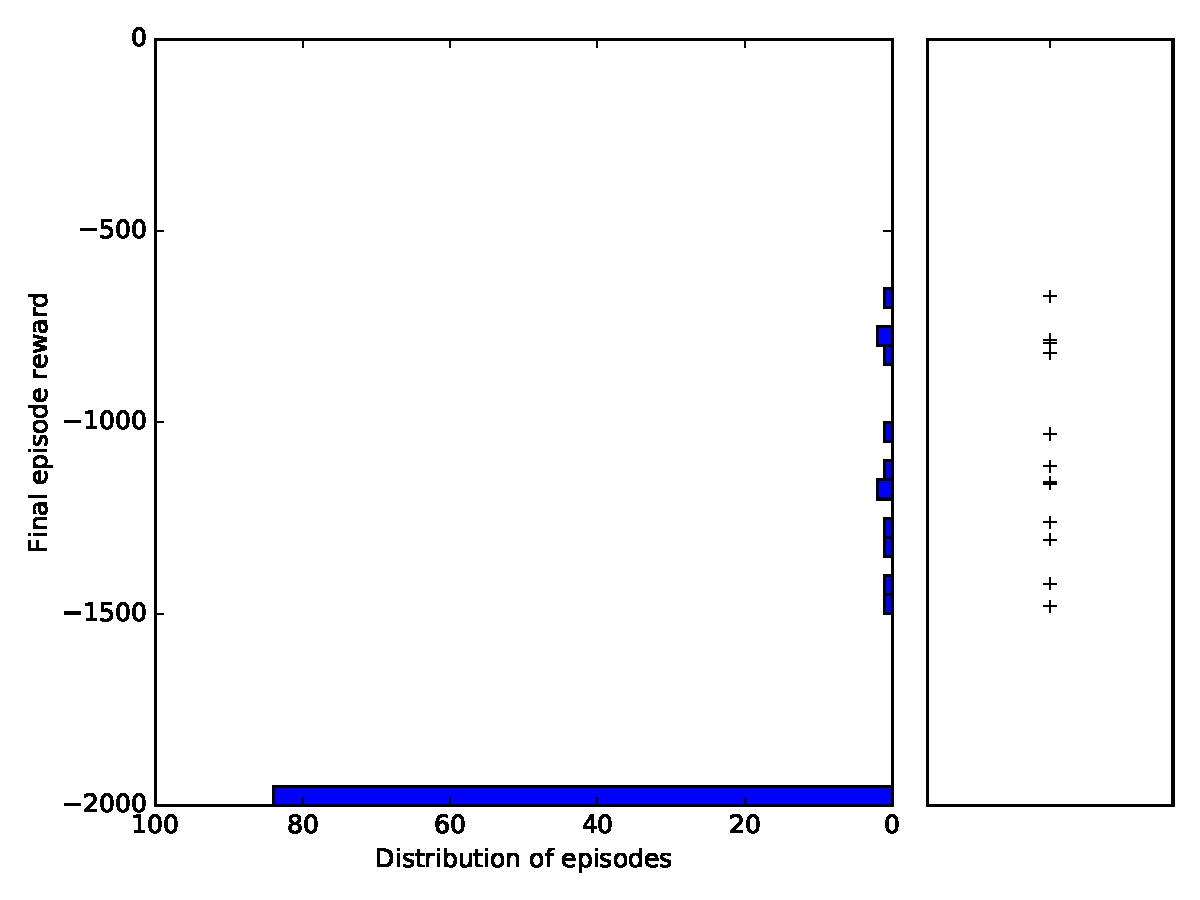
\includegraphics[width=0.49\linewidth]{fig/distrib1_cunseen.pdf}}
	\subfloat[][Trials of 2 episode]{
		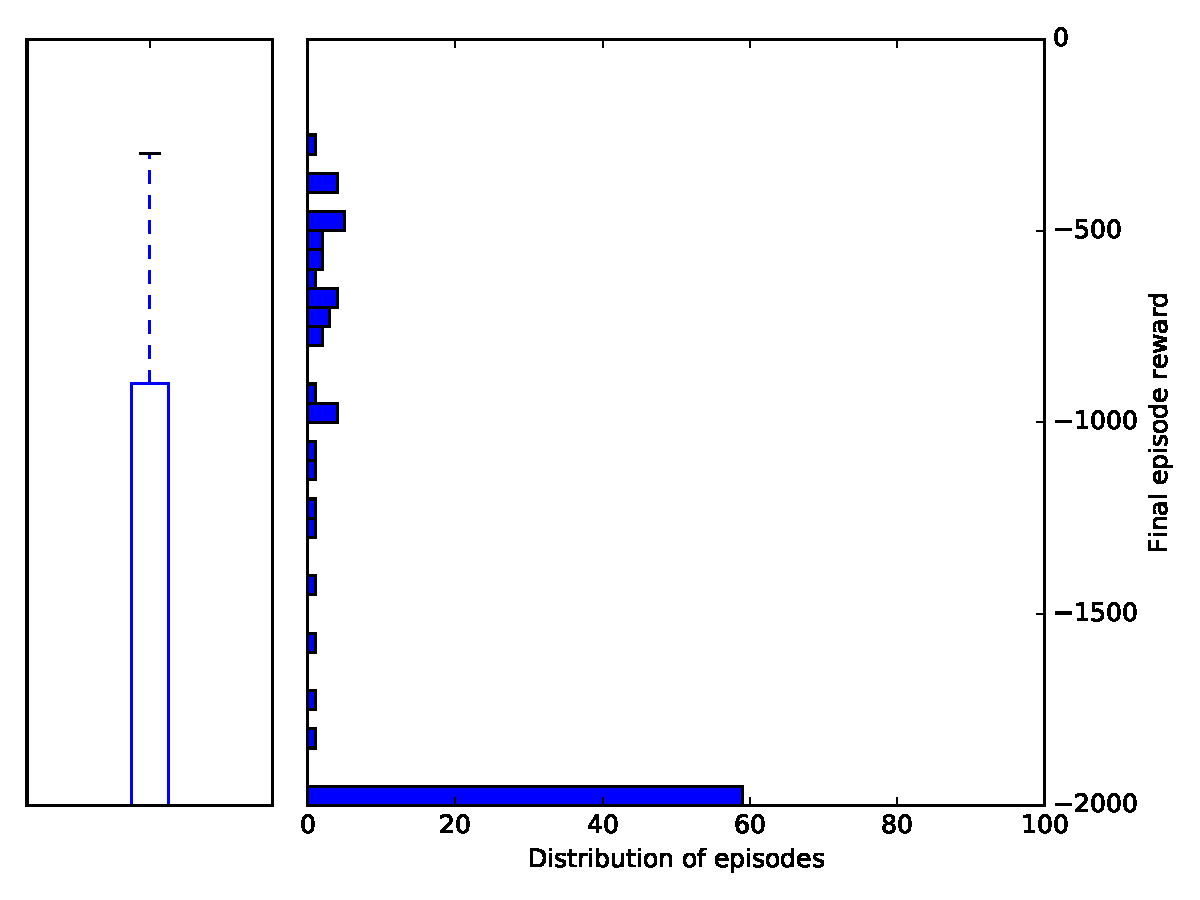
\includegraphics[width=0.49\linewidth]{fig/distrib2_cunseen.pdf}}
	\caption{Distribution of the total reward obtained during final episodes
	for trials of different lengths for experiment 2}
	\label{fig:distrib_cunseen}
\end{figure*}


\subsection{Experiment 1}
The first experiment will compare the performance of our agent in settings
that it has seen during training on trials of 1 and 2 episodes. We will only
look at the distribution of obtained rewards for final episodes (the second 
episode in the dual-episode setting and the first and only episode in the
single-episode setting) as the nonterminal episodes are considered to be the 
"learning" episodes.

We fix the agent's weights after training for this experiment. Just to make sure
we are clear, we expect the agent to show a learning behaviour after training,
meaning that its reward per episode should increase as it plays more episodes.
The learning policy should be encoded in the agent's weights.

The agent plays 192 trials for each setting (single-episode and dual-episode).
The parameters are sampled uniformly from the same distributions as the training.

As Figure~\ref{fig:distrib} shows, letting the agent play for 2 episodes
leads to generally higher reward. Although the difference is slight, 
in this experiment, failed episodes (failing
to swing the second link high enough within 2000 timesteps) occur in the
single-episode setting only.

The graph of Figure~\ref{fig:distrib} lacks the "knowledge gain" information.
Even if it shows that failures stop occuring, we don't know yet exactly how
much better the second episode is compared to the first one.

If we look at the distribution of reward difference between the first
and second episode of dual-episode trials (Figure~\ref{fig:reward_diff}), we 
see that in general, although a majority of differences are negligible,
second episodes improve on their respective first episodes - some of them
reaching the goal as much as 1500 timesteps faster than the first episode. These
are likely to be the failed first episodes followed by successful episodes
after the agent gained knowledge about its environment.

\subsection{Experiment 2}
One of the goals of meta reinforcement learning is to train agents that are
ready to handle new and unseen situations. Testing our meta-learning agent
on situations it has seen during training can give us some insight into
its behaviour, but our analysis would not be complete if we did not test it 
in unknown situations.
\begin{figure*}
	\centering
	\subfloat[][Trials of 1 episode]{
		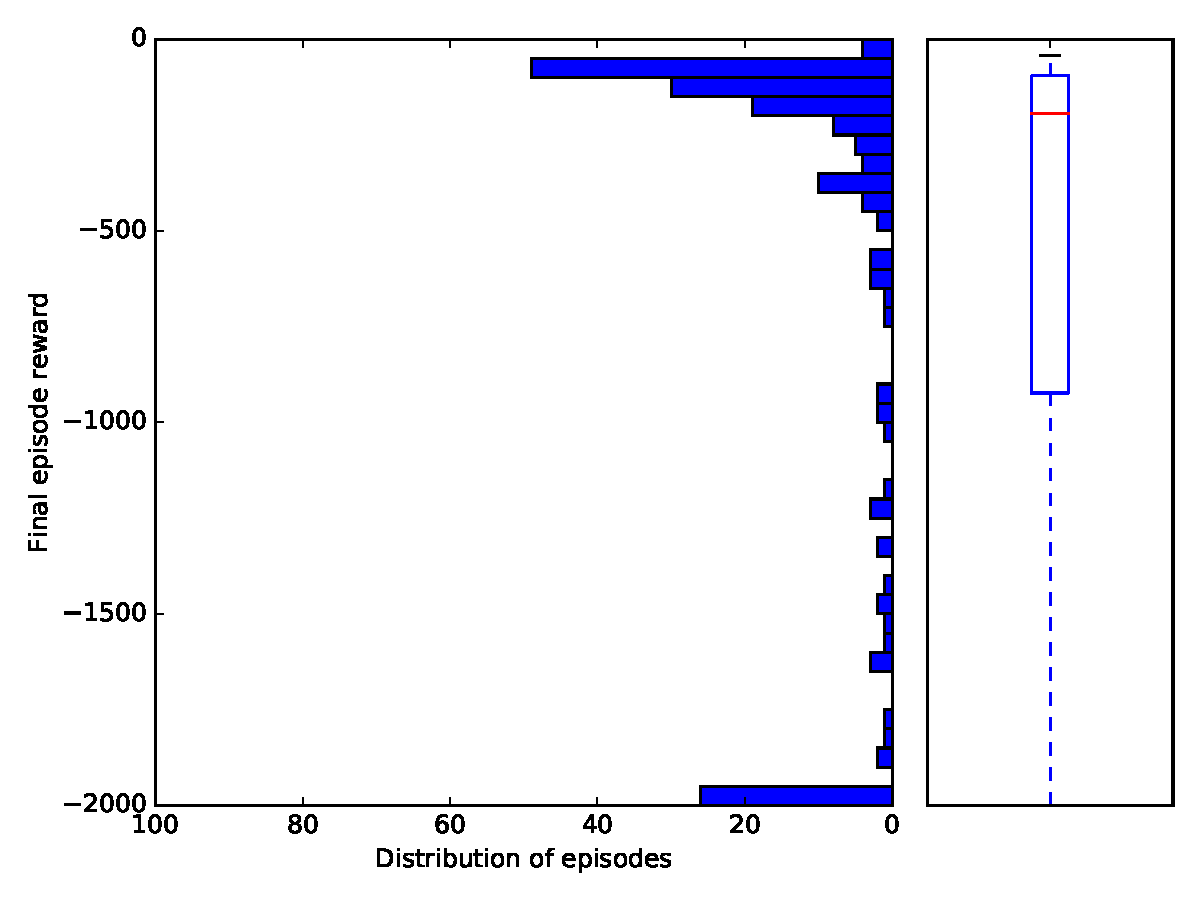
\includegraphics[width=0.49\linewidth]{fig/distrib1_mask.pdf}}
	\subfloat[][Trials of 2 episode]{
		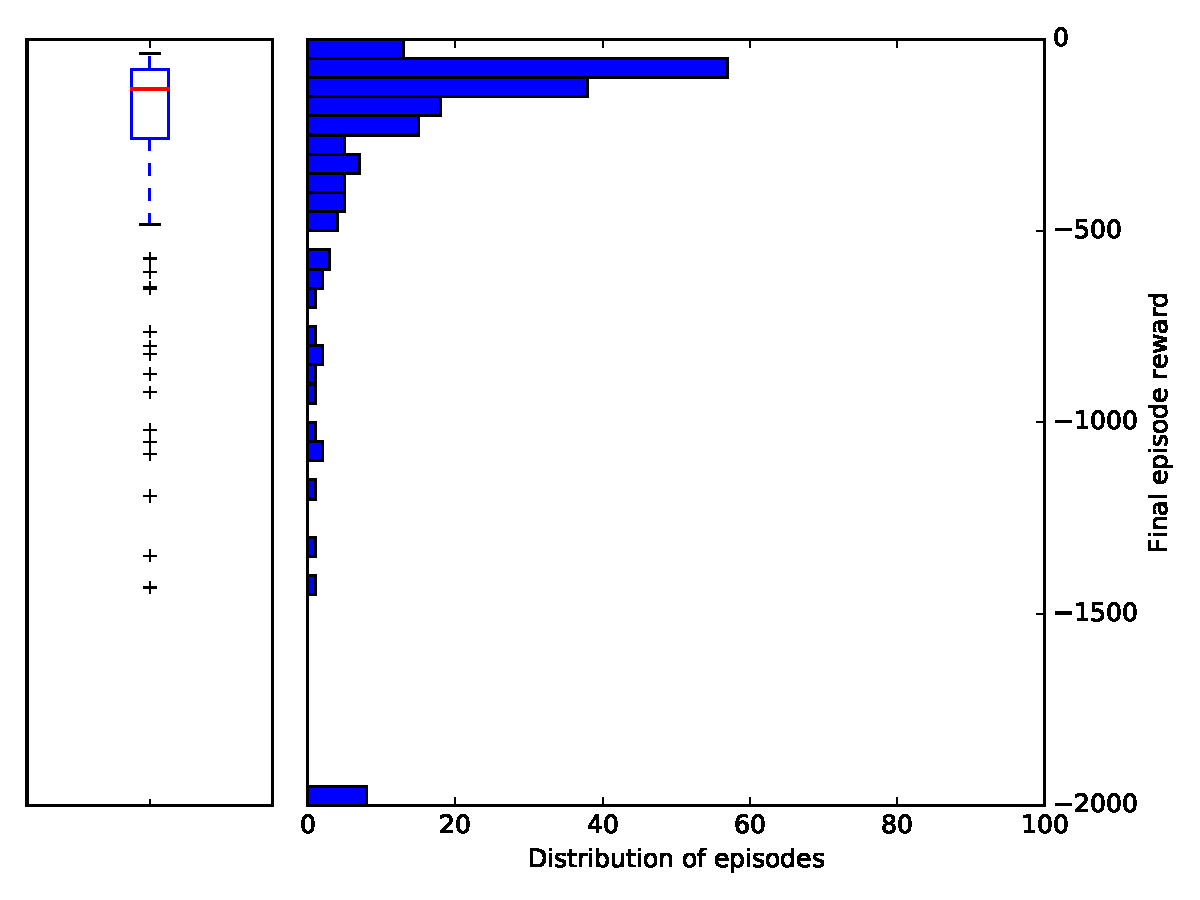
\includegraphics[width=0.49\linewidth]{fig/distrib2_mask.pdf}}
	\caption{Distribution of the total reward obtained during final episodes
	for trials of different lengths for experiment 3}
	\label{fig:distrib_mask}
\end{figure*}

\begin{figure}[h]
	\centering
	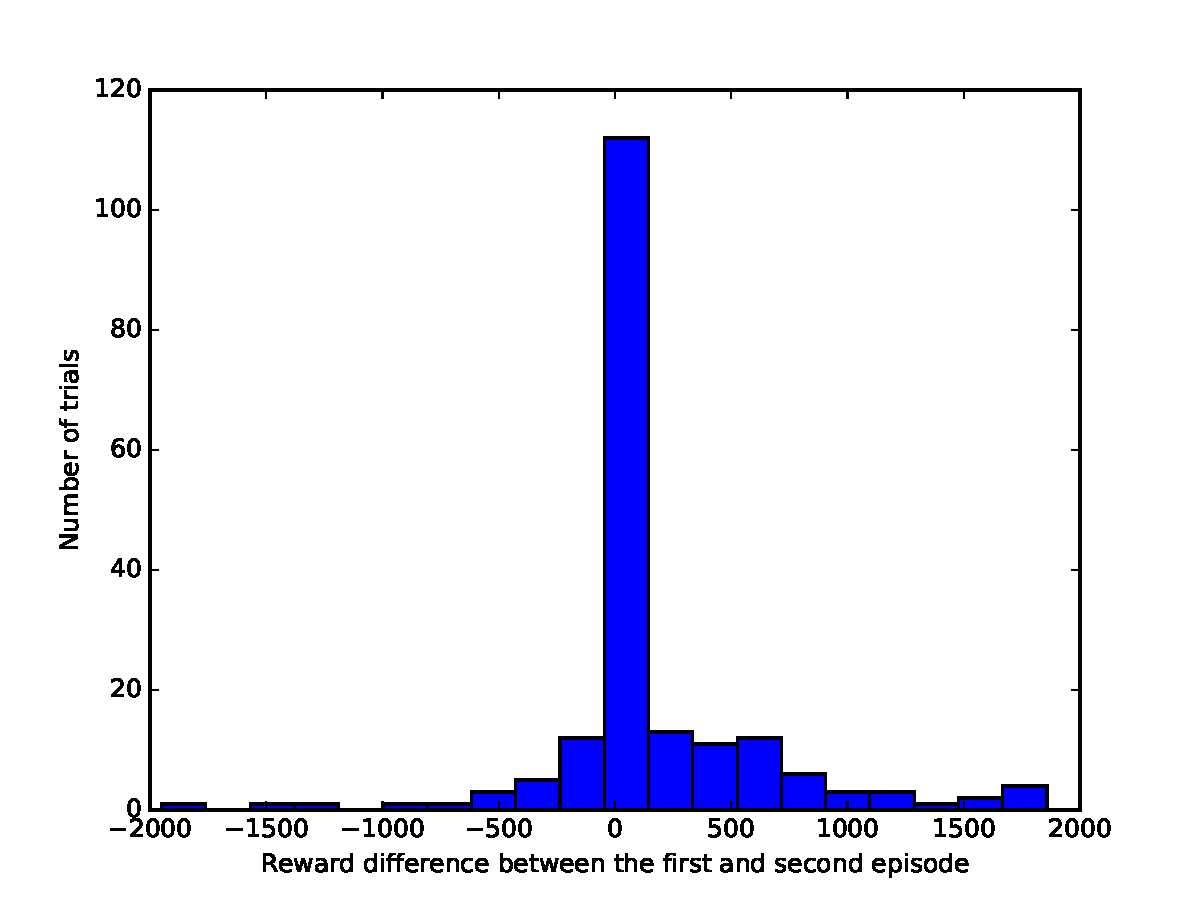
\includegraphics[width=\linewidth]{fig/reward_diff_mask.pdf}
	\caption{Distribution of the reward difference between the first
	and the second episode of a dual-episode trial for experiment 3}
	\label{fig:reward_diff_mask}
\end{figure}


In this experiment, we will try to get a grasp of the performance of our agent
in completely unseen settings, where:
\begin{itemize}
	\item the length for each pole is sampled uniformly and independently 
		between 2 and 3:
		$l \sim \mathcal{U}[2, 3] $
	\item the mass for each pole is sampled uniformly and independently 
		between 1 and 2:
		$m \sim \mathcal{U}[1, 2] $
\end{itemize}

The setting of the experiment is otherwise the same as the one presented for
experiment 1.

The results however are dramatically different (see
Figure~\ref{fig:distrib_cunseen}). Instead of mostly
achieving good results, both the agent having been trained in the single-episode
and dual-episode settings seem to mostly fail. The agent trained
in the dual-episode setting still seems to be the best performer, failing thrice
less than the agent trained in the single-episode setting (37 episodes
achieving a reward higher than -2000 versus 12).

Such a large number of failures could be attributed to the fact that the
parameters used for this experiment are outside of the range presented to
the agent during training and thus may require a wholly new strategy to be
deployed in order to reach high rewards.

The difference between episode 1 and episode 2 presents a similar distribution
as the one shown in experiment 1 (see Figure~\ref{fig:reward_diff_cunseen}). 
For a majority of trials, the second episode
neither improves or deteriorates reward, but there is a non-negligible group
of trials in which quite a significant increase is achieved.

\subsection{Experiment 3}
So far, we have only tried tuning intrinsic parameters of the environment. This
kept both the setting of experiment 1 and the setting of experiment 2 quite
similar. In this experiment, we will explore how tampering with the
observation process rather than the environment dynamics affects the performance
of our agents. Hence the lengths and masses for each link are sampled 
uniformly and independently from the values on which the agent has been trained.

For each trial, we select at random one of the values of the observation vector
which will be masked out throughout the whole trial; meaning that the
observation for this value will always be 0. 

Figure~\ref{fig:distrib_mask} shows the result of this experiment. Once again,
even though the general performance for both the single-episode and the
dual-episode setting is lower than the one presented in experiment 1, the
agent trained on trials of two episodes gets the upper hand; both by
having more episodes with a higer reward but also by failing 20 trials less
than the agent trained on a single episode.

The distribution of reward difference between the first and second episode
of dual-episode trials looks similar to the ones we have seen before: a
majority of negligible differences, and visibly more gains than losses.

\section{Conclusions}
We have presented a simple reward shaping method to allow the meta-learning
setup presented by \cite{learningtorl} and \cite{fastrlviaslowrl} to be applied
to problems with a continuous state space and a constant reward given at
each timestep such as Acrobot (on which were run all the experiments of this
paper) and CartPole.

We analysed the performance of a meta-learning agent and the gains it realised
by playing two episodes by learning from its experience in the first episode.
A distribution of Acrobot problems was generated by changing the link lenghts
and masses, inherently changing the difficulty of the game and the strategy
needed to be deployed to reach high rewards.\\

The analysis was carried on three settings:
\begin{itemize}
	\item the training setting
	\item a test setting, using weight and length values which were
		outside of the range of values used in training
	\item the training setting but with a mask randomly zeroing one of the
		four observation values for the length of a trial.
\end{itemize}
In the three settings, playing two episodes proved to be beneficial for the 
agent and the reward obtained in the second episodes of trials was mostly
equal or better than the reward obtained in the first episodes.\\

We firmly believe that the generalisation power of the meta-learning agent
and its resilience to changes in the rules of the game could be further
exploited by using it on more complex problems in which learning cannot occur
within one episode (which was the case for some of our experiments, making
the increase of performance between first and second episodes sometimes slight).

\paragraph{Implementation} The implementation of the meta-learning A2C agent
and its training process is available online and uses 
Tensorflow \citep{tensorflow} and OpenAI Gym \citep{gym}:\\
\url{https://github.com/fhennecker/meta-rl-acrobot}
\footnotesize
\bibliographystyle{apalike}
\bibliography{report}


\end{document}
